\documentclass[dvipdfmx,a4paper]{jsarticle}
\usepackage{amsmath,amssymb}
\usepackage{amsthm}
\usepackage{bm}
\usepackage[dvipdfmx]{graphicx}
\usepackage{ascmac}
\usepackage{subfigure}
\usepackage{verbatim}
\usepackage{wrapfig}
\usepackage{makeidx}
\usepackage[dvipdfmx]{hyperref}
\usepackage{setspace}
\usepackage{color}
\usepackage{listings}
\usepackage{cleveref}
\usepackage{mathtools}
\usepackage{framed}
\usepackage[textwidth=50zw,lines=46]{geometry}
\usepackage{here}

\usepackage{listings, jlisting, color}
\definecolor{OliveGreen}{rgb}{0.0,0.6,0.0}
\definecolor{Orenge}{rgb}{0.89,0.55,0}
\definecolor{SkyBlue}{rgb}{0.28, 0.28, 0.95}
\lstset{
  language={C++}, % 言語の指定
  basicstyle={\ttfamily},
  identifierstyle={\small},
  commentstyle={\smallitshape},
  keywordstyle={\small\bfseries},
  ndkeywordstyle={\small},
  stringstyle={\small\ttfamily},
  frame={tb},
  breaklines=true,
  columns=[l]{fullflexible},
  numbers=left,
  xrightmargin=0zw,
  xleftmargin=3zw,
  numberstyle={\scriptsize},
  stepnumber=1,
  numbersep=1zw,
  lineskip=-0.5ex,
  keywordstyle={\color{SkyBlue}},     %キーワード(int, ifなど)の書体指定
  commentstyle={\color{OliveGreen}},  %注釈の書体
  stringstyle=\color{Orenge}          %文字列
}

\begin{document}

\title{課題演習C3\quad レポート (2回目) }
\author{0500-34-0042\quad 大平 達也}
\date{2025/01/23}
\maketitle

\section{目的}
前回のレポートから, 大きく次の2つの進捗があった。
\begin{itemize}
  \item 参照星のクオリティーチェック
  \item トランジットモデルとデータの比較
\end{itemize}
それぞれについて以下で報告する。

\section{参照星のクオリティーチェック}
前回のレポートで述べた手法で参照星を選んだ。今回は, それらの参照星のクオリティーチェックを行った。
\subsection{手法}
まず, 参照星のフラックスを平均を用いて各参照星のフラックスを補正した。
その後, それぞれの参照星の等級の分散を計算した。
最後に, フラックスの変化が1\%を超えるようであれば, フラックスの変化が1\%程度の, 最低限のビンで移動平均を取った。

コードは (計算しただけであるので) 省略する。

\subsection{結果}
まず, 参照星のfinding chartを図\ref{fig:finding_chart}に示す。そして, これら参照星の等級の分散と標準偏差を表\ref{tab:compstars}に示す。

ここで, フラックス変化が$\Delta F/F$のときの等級の変化$\Delta m$は, 
$$\Delta m= -2.5\log(1+\Delta F/F)\simeq -2.5\times \dfrac{1}{\ln 10}\dfrac{\Delta F}{F}\simeq -1.09\dfrac{\Delta F}{F}$$
であるため, フラックスの変化が1\%程度であれば, 等級の変化は約0.01等級程度である。

そのため, 観測データの品質は十分であると考えられる。

\begin{figure}[H]
  \centering
  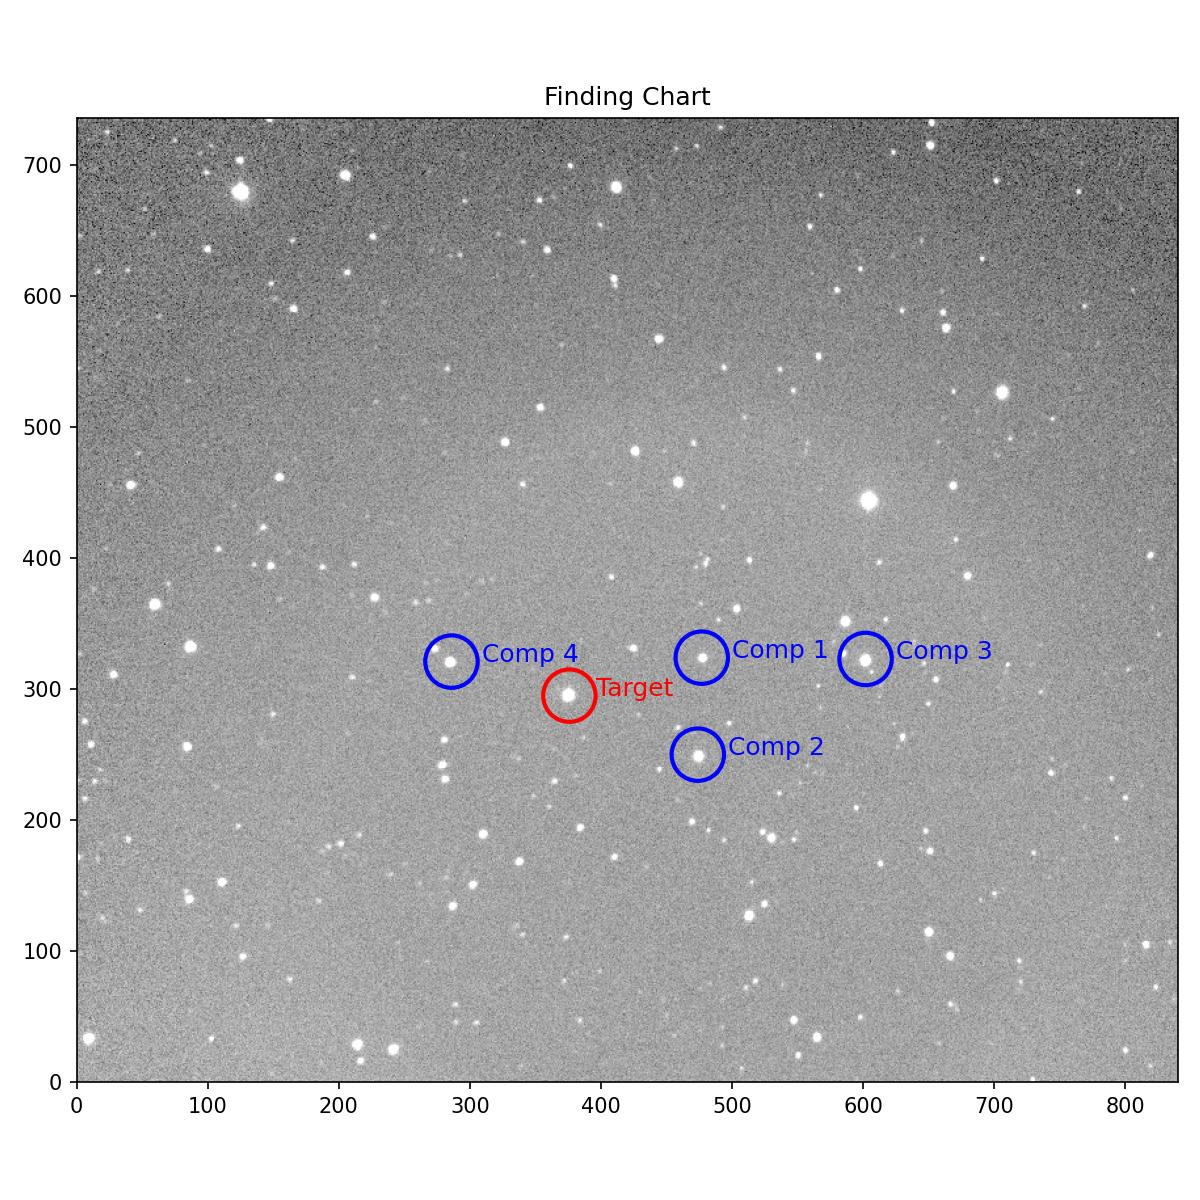
\includegraphics[width=0.65\textwidth]{./fig/finding_chart.png}
  \caption{参照星のfinding chart}
  \label{fig:finding_chart}
\end{figure}

\begin{table}[htbp]
  \centering
  \caption{参照星の分散と標準偏差}
  \label{tab:compstars}
  \begin{tabular}{c c c}
  \hline
  Comp & Variance & StdDev \\
  \hline
  1 & 0.00011 & 0.01028 \\
  2 & 0.00006 & 0.00782 \\
  3 & 0.00005 & 0.00693 \\
  4 & 0.00016 & 0.01249 \\
  \hline
  \end{tabular}
\end{table}

\section{トランジットモデルとデータの比較}
前章で品質を確認した参照星を用いて, トランジットの光度曲線を作成する。また, カタログから恒星系のパラメータを取得し, トランジットモデルを作成した。これらを重ねてプロットする。
\subsection{コード}

Python コードを掲載する。なお, パラメータは, \cite{Kabath2022}に従った。

実装の方針としては, トランジットモデルの計算の際に, トランジット中心時間をユリウス日で与え, 最後にdatetimeに変換することで, 観測データとトランジットモデルの時間を合わせた。また, 縦軸は, 観測データから補正したフラックスの, 最後の50点の中央値を1とする相対値を取った。
\begin{lstlisting}[caption=トランジットモデル計算およびプロット用のコード, label=model, language=Python]
    dt = datetime.datetime(2024, 11, 11, 21, 22, 00)

    # dt をユリウス日に変換
    t = Time(dt, scale='utc')
    t0_jd = jd_value
    
    # Transit parameter 設定
    params = batman.TransitParams()
    params.t0 = t0_jd        # トランジット中心を JD で設定
    params.per = 2.056014
    params.rp = 0.1224
    params.a = 6.220
    params.inc = 90.0
    params.ecc = 0.0
    params.w = 90.0
    params.u = []           
    params.limb_dark = "uniform"
    
    time_jd = np.linspace(params.t0 - 0.07, params.t0 + 0.07, 5000)
    
    # トランジットモデルの計算
    m = batman.TransitModel(params, time_jd)
    flux_model = m.light_curve(params)
    
    # datetimeに変換しておく
    time_datetime = Time(time_jd, format='jd').to_datetime()
    
    # ここからはデータのプロット
    times_jst_naive = [dt.replace(tzinfo=None) if dt is not None and not isinstance(dt, float) else dt for dt in times]
    
    # データをDataFrameに変換
    df = pd.DataFrame({
        'Time': times_jst_naive,
        'Flux_Norm': norm_fluxes
    })
    
    # 'Time'をDatetimeIndexに設定
    df.set_index('Time', inplace=True)
    time_array = df.index.to_numpy()
    
    # 光度曲線のプロット
    fig, ax = plt.subplots(figsize=(10, 6))
    plt.plot(time_array, df['Flux_Norm'], 'o', markersize=3, alpha=0.3, color='black', label="data")
    plt.plot(time_datetime, flux_model, color='black', lw=3, label="model")
    ax.xaxis.set_major_formatter(mdates.DateFormatter('%H:%M'))
    # plt.gca().invert_yaxis()
    plt.xlabel('Time')
    plt.ylabel('Flux [Rel.]')
    plt.title('TOI-1516 Light Curve')
    plt.grid(True)
    plt.show()
    fig.savefig('light_curve_fit.png')
\end{lstlisting}

\subsection{結果}
図\ref{fig:transit_model}に, 光度曲線を示す。モデルの曲線が概ねデータの範囲に収まっていることが確認された。嬉しい。

\begin{figure}[H]
  \centering
  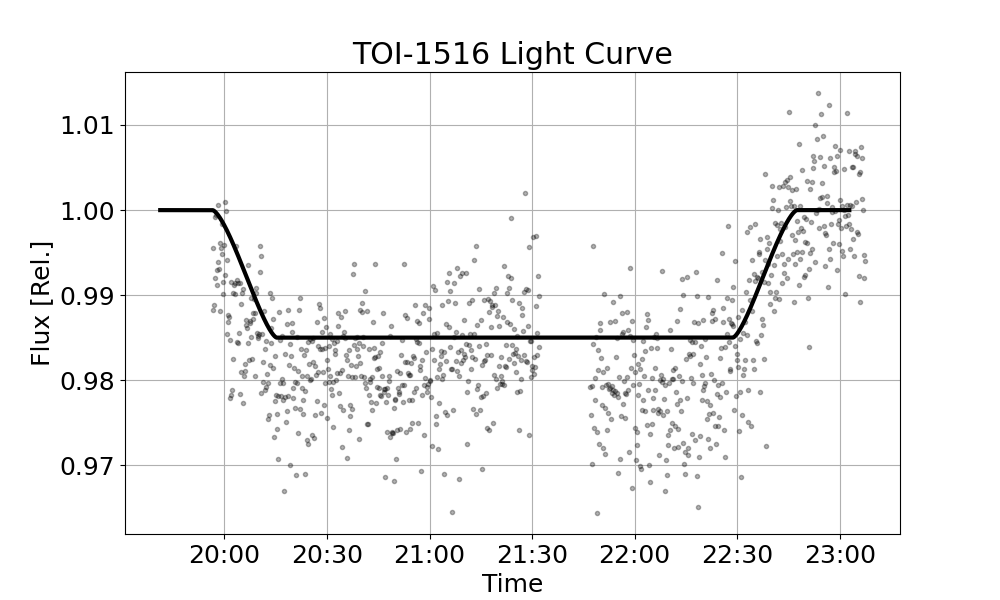
\includegraphics[width=0.9\textwidth]{./fig/light_curve_fit.png}
  \caption{TOI-1516の光度曲線}
  \label{fig:transit_model}
\end{figure}

\begin{thebibliography}{9}
\bibitem{Kabath2022}
Kabáth, P., Chaturvedi, P., et al.\ 
2022, 
\textit{Monthly Notices of the Royal Astronomical Society}, 
513(4), 5955--5972.
\end{thebibliography}
\end{document}